\chapter{Dense Matrix}

In this chpater, We will discuss implementation about dense matrix. Dense matrix is a matrix, Which have mostly element are non zero. We will implement matrix- vector, matrix multiplication and matrix addition and subtraction in CPU and OCCA.

\section{Dense matrix - vector multiplication}
\subsection{Introduction}
Matrix vector multiplication computes the product of matrix and vector. We can perform multiplications between a matrix and vector when number of columns of matrix equal number of rows of vector. In mathematical term m*n dimensional matrix can be multiplied only n dimensional vector.The theoretical operation is shown below, matrix-vector multiplication output is m*1 dimensional vector.\\
Input data: dense matrix A
 of size m-by-n (with entries $a_{ij}$
), its vector cofactor x
 of dimension n (with components $x_i$
).

Output data: vector y
 of dimension m (with components $y_i$
).

Formulas of the method:
\begin{equation}
	y_i = \sum _{j=1}^{n} a_{ij}x_j \quad   i \in [1...m]
\end{equation}

%There also exists a block version of the method. However, this description treats only the pointwise version.
The basic idea with visualisation as below:
\begin{center}
	
\end{center}
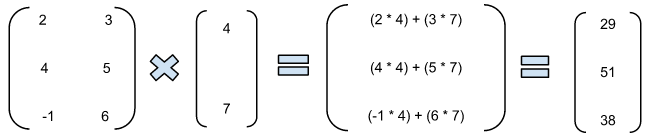
\includegraphics[width=12cm, height=2cm]{Chapters/matrix-vector-multiplication.png}
\captionof{figure}{matrix vector multiplication}
%\centerline{ 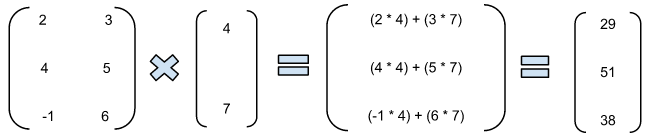
\includegraphics[width=12cm, height=2cm]{Chapters/matrix-vector-multiplication.png}}
\subsection{C++ implementation}
The C++ implementation is the most basic implementation. The idea is below\\

\begin{lstlisting}[language=C, caption=matrix vector multiplication in CPU/C++]
	we have m*n dimensional matrix
	for i < m;i++
		for j < n;j++
			result_vector[i] += matrix[i*n+j]*vector[j]
\end{lstlisting}

Listing 2.1 each iteration of the for loops, the code computes the product of two elements of matrix and vector and add the result. So the time complexity of the entire multiplication is $O(n^2)$, if we have matrix size n-by-n.




\subsection{OCCA implementation}
The OCCA utilises the data parallelism in matrix - vector multiplication.\\
\begin{lstlisting}[language=C, caption=matrix vector multiplication in OCCA]
	we have m*n dimensional matrix
	for i < m; i++;@tile(16, @outer, @inner)) // Work-group implicit loops
		for j < n;j++
			result_vector[i] += matrix[i*n+j]*vector[j]
\end{lstlisting}
In Listing 2.2, An additional tile tag was introduced to facilitate kernel development due to many kernels only requiring the use of simple bounds and iteration strides. The tile tag, tiling for-loops as one and two dimensional sets of inner/outer loops. The tile(16) assign the working dimension. In this example it assign the working dimension is 16. 
\subsection{OCCA vs CPU}

\begin{center}
	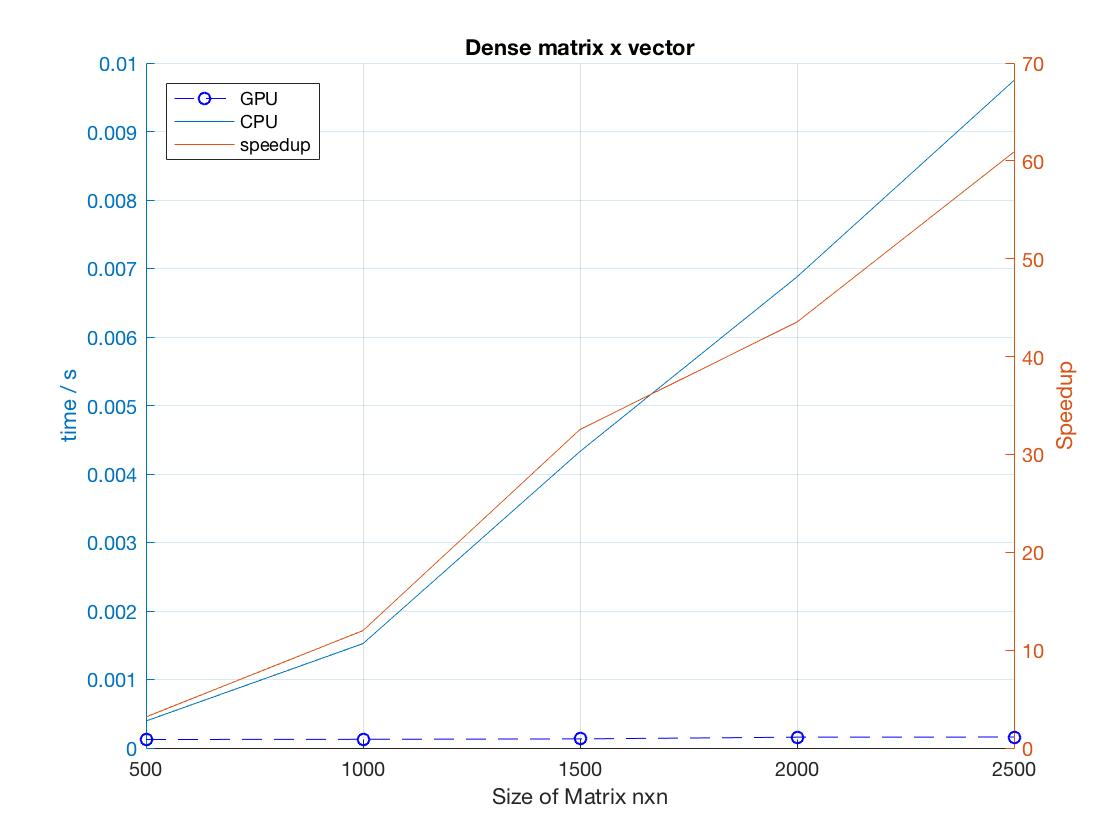
\includegraphics[width = 12cm]{chapters/dense_matrix_vector.jpg}
	\captionof{figure}{compare OCCA vs CPU performance}
	\label{img:1}
\end{center}

As we can see in figure \ref{img:1} OCCA always faster than CPU. If matrix and vector size is bigger than OCCA perform better than CPU.





\section{Dense matrix-matrix  multiplication}
\subsection{Introduction}
Matrix multiplication computes the product of two matrices. The theoretical operation show below, where matrix A and matrix B are the input matrices and produce the output matrix.\\
\begin{center}
	\includegraphics[width = 10cm]{../Matrix_multiplication}
	\captionof{figure}{matrix multiplication visualisation }
\end{center}

Let C is output matrix then mathematical formulation of the equation is
\begin{equation}
	C_{ij}=a_{i1}b_{1j}+\cdots +a_{im}b_{mj}=\sum _{k=1}^{m}a_{ik}b_{kj}
\end{equation}
for i = 1, ..., n and j = 1, ..., p.\\
That is, the entry $C_{ij}$ of the product is obtained by multiplying term-by-term the entries of the $i^{th}$ row of A and the $j^{th}$ column of B and summing these m products. In other words, $C_{ij}$ is the dot product of the $i^{th}$ row of A and the $j^{th}$ column of B.

\subsection{C++ implementation}
The C++ implementation is the most basic implementation. The pseudo code is below
\begin{lstlisting}[language=C, caption=matrix multiplication in CPU/C++]
	we have  m*n and n*m dimensional matrices
	for i < m; i++
		for j <m; j++
			for k < n;k++
				result[i][j] += A[i][k]*B[k][j]
\end{lstlisting}
In Listinig 2.3 , each iteration of the for loops, the code computes the product of two elements from matrix A and matrix B and add the product to the result from previous iteration of the loops. For example m by m square matrix to compute the element in result matrix, the CPU performs m multiply operations and n-1 sum operations. So the time complexity of entire multiplication there are $O(n^3)$ multiply operations and $O(n^2)$ sum operations.

\subsection{OCCA implementation}
The OCCA utilises the parallelism in matrix multiplication. The kernel launches $n^2$ thread blocks for an n by n square matrix multiplication. Each block does the multiplication of the row of matrix A and column of matrix B. Each thread block computes the product of one element of A and one element of matrix B.\\
We have pseudo code for okl as below
\begin{lstlisting}[language=C, caption=matrix multiplication in OCCA]
	we have  m*n and n*m dimensional matrices 
	for k < n; k++
		for o1 < m; o1+=16;@outer
			for o0 < m; o0+=16; @outer
				for y= o1; y <o1+16;y++;@inner
					for x = o0; x <o0+16;x++;@inner
						result[i][j] += A[y][k]*B[k][x]
	
\end{lstlisting}
Listing 2.4, The start, end and stride used in the outer and inner loops to support argument based variables and the working dimensions are resolved at run-time. Currently working dimensions must constant across on all the inner-loops defined in outer loop. In this example k will increment linearly but x and y will work in working dimensions. In this case our working dimensions is 16. We explain further about inner loop in chapter 1 \ref{txt:innerOuterloop} .
\subsection{OCCA vs CPU}
\begin{center}
	\includegraphics[width = 10cm]{../matlab/dense_matrix.jpg}
	\captionof{figure}{comparison OCCA vs CPU performance}
	\label{img:2}
\end{center}
%\centerline{ \includegraphics[width = 10cm]{../matlab/dense_matrix.jpg}}
To test the performance of CPU and GPU. We take two array of size m-by-n and compute the matrices multiplication. We use the square matrices, the dimensions of the matrices start from 500 by 500 to 2500 by 2500. The throughputs of the CPU and GPU as shown above \ref{img:2} . We use the semiology for plotting in Matlab. If size of matrices is small than the CPU perform better than GPU. But the large the size, the CPU gets poor performance.\\
	The GPU memory transfer overhead has negative impact on the overall GPU performance. GPU memory transfer overhead cause the GPU overall throughput to be 10x lower than the GPU kernel overhead. 



\section{Dense matrix - matrix addition \& subtraction}
\subsection{Introduction}
We can perform addition or subtraction operations over 2 matrices. In this, we add element at position i*j in matrix A with element at the same position in matrix B. We can perform addition or subtraction operations only on same dimension matrices.\\
Let C is output matrix then mathematical formulation of the equation is
\begin{equation}
	C_{ij}=a_{ij} \pm b_{ij}
\end{equation}

for i = 1, ..., n and j = 1, ..., p.\\
That is the entry $C_{ij}$ is the sum or subtracion of the $i^{th}$ row and $j^{th}$ column of A and the $i^{th}$ row and $j^{th}$ column of B.\\
\begin{center}
	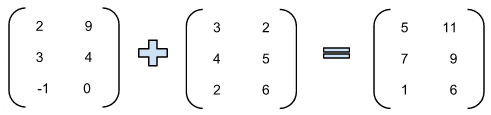
\includegraphics[width = 10cm]{Chapters/matrix-matrix-addition.png}
	\captionof{figure}{matrix addition}
\end{center}

\subsection{C++ implementation}
The C++ implementation is easy for the addition or subtraction. We can use the same function for the both operations. The pseudo code is below
\begin{lstlisting}[language=C, caption=matrix addition or subtraction in C++]
	we have m*n dimension both matrices
	if addition 
		operation = 1
	else 
		operation = -1
	for i < m; i++
		for j < n; j++
			result [i][j] = A[i][j]+(operations * B[i][j])
\end{lstlisting}
Listing 2.5, In each iteration the code will add one element of ij position of A matrix with one element of ij position of B matrix. For the subtraction we just multiply -1 with element of B matrix. And we save the result on same position in result matrix. The time complexity of this code is O($m*n$). If m is equal to n than we can say $O(n^2)$. 
\subsection{OCCA implementation}
A simple approach to compute addition or subtraction of two matrices on a GPU. The OKL pseudo code is below 
\begin{lstlisting}[language=C, caption=matrix addition or subtraction in OCCA]
	we have m*n dimension both matrices
	for o1 < m; o1+=16;@outer
			for o0 < m; o0+=16; @outer
				for y= o1; y <o1+16;y++;@inner
					for x = o0; x <o0+16;x++;@inner
						result[x][y] = A[x][y]+(operation * B[x][y])
\end{lstlisting}
Listing 2.6, The start, end and stride used in the outer and inner loops to support argument based variables and the working dimensions are resolved at run-time. Currently, working dimensions must constant across on all the inner-loops defined in outer loop. In this example x and y will work in working dimensions. In this case our working dimensions is 16. As we can see we are increment o0 and o1 by 16 and run x and y from o0 and o1 to o0+16 and o1+16. Which divide the work in group items.
\subsection{OCCA vs CPU}
\begin{center}
	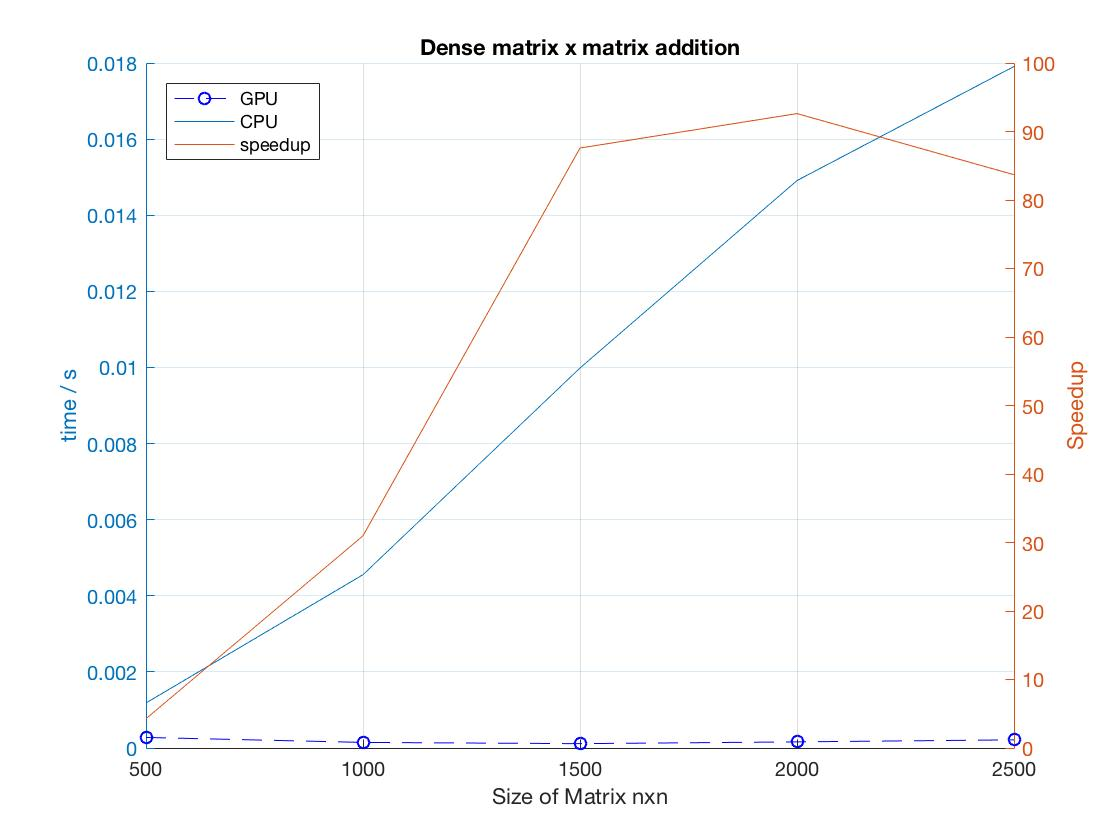
\includegraphics[width = 8cm]{Chapters/matrix_addition.jpg}
	\captionof{figure}{comparison OCCA vs CPU performance}
\end{center}
To test the performance of CPU and OCCA. We take two array of size m-by-n and compute the addition of the matrices. We use the square matrices, the dimensions of the matrices start from 500 by 500 to 2500 by 2500. The throughputs of the CPU and OCCA as shown above. We use the semiology for plotting in Matlab. If size of matrices is small than the CPU perform better than OCCA. But the large the size, the CPU gets poor performance.